\documentclass{article}

\usepackage[T1]{fontenc}
\usepackage[utf8]{inputenc}
\usepackage[russian]{babel}
\usepackage{amsmath}
\usepackage{array}
\setlength{\parskip}{10pt}
\usepackage[hidelinks]{hyperref}% Отступ между абзацами
\usepackage{graphicx}
\usepackage[most]{tcolorbox}
\usepackage{listings}
\usepackage{xcolor}
\usepackage{ulem}


\lstset{
  language=Python, % Замените на нужный язык программирования
  basicstyle=\ttfamily\footnotesize, % Основной стиль шрифта
  keywordstyle=\color{blue}\bfseries, % Цвет ключевых слов
  commentstyle=\color{gray}\itshape, % Стиль комментариев
  stringstyle=\color{red}, % Цвет строк
  numbers=left, % Нумерация строк (left, right, none)
  numberstyle=\tiny\color{gray}, % Стиль нумерации
  stepnumber=1, % Шаг для нумерации строк
  numbersep=10pt, % Расстояние между кодом и номерами строк
  backgroundcolor=\color{lightgray!20}, % Фон кода
  frame=single, % Рамка вокруг кода (можно убрать)
  tabsize=4, % Размер табуляции
  captionpos=b, % Подпись под кодом (b - ниже, t - выше)
  breaklines=true, % Перенос длинных строк
  breakatwhitespace=true, % Перенос строк только между словами
  showspaces=false, % Не показывать пробелы
  showstringspaces=false % Не показывать пробелы внутри строк
}

\newtcolorbox{mychatbox}[2][]{
    colback=blue!5!white, % Цвет фона сообщения
    colframe=blue!75!black, % Цвет рамки сообщения
    width=\linewidth, % Ширина блока
    sharp corners, % Прямые углы
    boxrule=0.5mm, % Толщина рамки
    fontupper=\small\itshape, % Шрифт текста
    title=#2, % Имя пользователя
    title style={font=\bfseries}, % Оформление имени
    #1 % Дополнительные параметры
}





\begin{document}

\title{Проект по Продвинутым Методам Машинного Обучения}
\author{Уколов Степан, Сиворакша Тимофей, Алиев Элвин, Валерий Ходжаев}
\date{18.12.2024}
\maketitle

\newpage
\tableofcontents

\newpage

\section{Введение}


\begin{mychatbox}[colback=red!5!white]{Пользователь}
сгенерируй смешную картинку для rag проекта по поиску домов для аренды
\end{mychatbox}

\vspace{1em}

\begin{mychatbox}[colback=green!5!white]{ChatGPT}
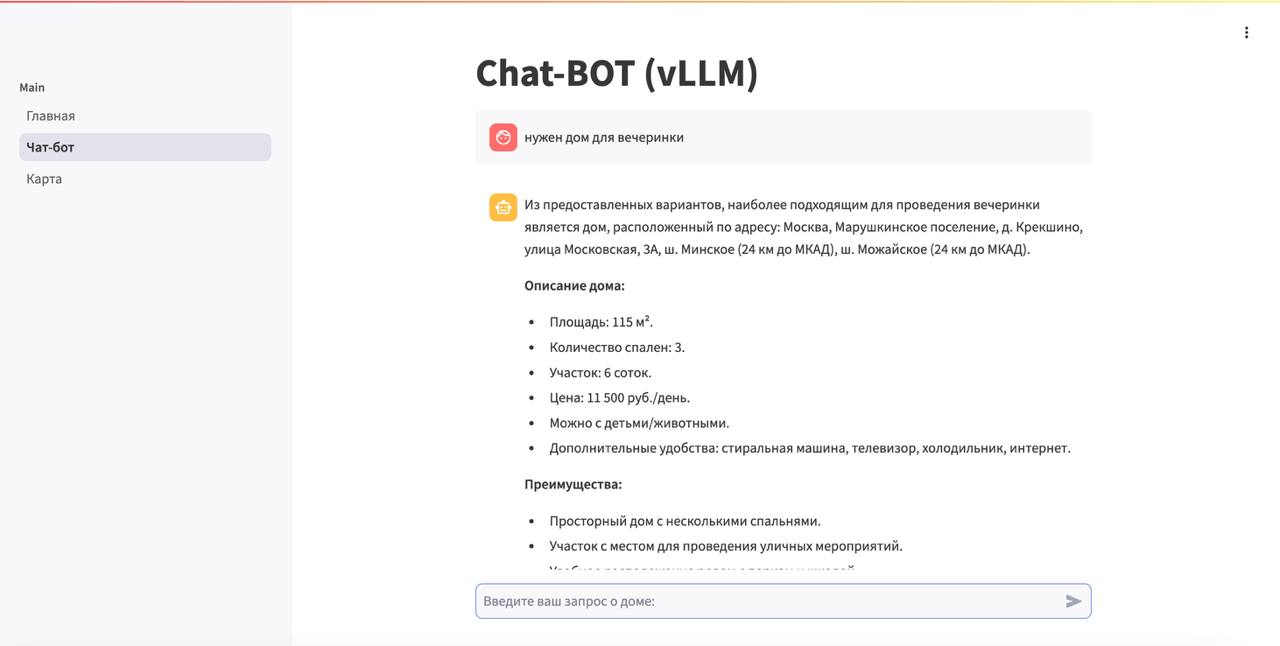
\includegraphics[width=0.5\textwidth]{1.jpg}
\end{mychatbox}

\\
\\
\\
\\

Бедные орги каждый год долго-долго выбирают дома на посвят( Мы решили, что так больше продолжаться не может: \sout{отменяем посвят} делаем супер-пупер RAG систему с возможностью быстрого и удобного подбора релевантных объявлений! Как говорится «Лофты размыли ценность посвята», пора решать эту проблему! 

\\

Хочеца введение ещё расписать, картинок по вставлять, но так уже лень… Тем более во время написания введения в гжк упал инет(


Проект посвящён обработке данных по объявлениям аренды загородных домов с платформы ЦИАН. Как говорится, начинали с простого анализа, а закончили риелторским стартапом. Но обо всём по порядку!


P.S.


В этой пдфке много разных гиперссылок на “жирном тексте” (не на заголовках) => не стесняемся, наводим курсор, пробуем тыкать



\newpage

\section{Сбор данных}

\subsection{Почему именно Циан?}

Изначально предполагалось парсить Авито, но тщетные N часов попыток дали понять, что Авито, скорее всего, настолько устали от всяких парсеров/скрэтчеров, что
\begin{enumerate}
    \item Понавтыкали своих cloudlfare, который еще и умеет смотреть на IP юзера, а не на имя агента в headers, да так, что всяких базовые библиотеки питона для обхода cloudlfare не лечат траблы.
    \item Повставляли на страницы элементы, которые грузят javascript контент, из-за чего нужны умные библиотеки для запросов, которые умеют рендерить такие штуки (eg. HTMLrequests, Selenium)
    \item Придумали сложную генерацию ссылок со вставкой параметров, что глаза вытекают
    \item Спрятали все обращения к своим API
\end{enumerate}


В то время как Циан оставили кнопочку на сайте <Скачать в $Excel$>, но увы, там стоит ограничение на 200 домов, к тому же кнопку можно нажимать раз в сутки. Мы же хотим получить базу побольше.
Как и Авито, Циан генерирует ссылку на страницу с домами в зависимости от введённых параметров на основной странице. Так как мы не хотим проводить посвят в квартире или где-то в Мурманске и, к сожалению, не будем брать дом на срок более одних суток, вбиваем нужные параметры, а сгенеренную ссылку берем за основную. Снова приятный сюрприз, ссылки страниц домов оставлены на самой странице внутри одних и тех же тегов. Да и сами ссылки страниц домов созданы по понятному принципу: cian + имя ареала (eg. odintsovo) + внутренний id сущности в базе Циана. Более того, Циан предлагает пользователю только активные объявления, в отличие от \sout{мат} дурацкого Авито.

\subsection{Парсер Циан}

Стэк джентльмена:
\begin{lstlisting}[language=Python, label=code:example]
from bs4 import BeautifulSoup
import requests  
import pandas as pd 
\end{lstlisting}


В целом Циан - френдли сервис для парсинга. Даже на тот факт, что юзер отправляет слишком много запросов, он отвечает не 427 статус кодом, разрывая конекшн, как большинство сайтов, а 429 кодом, в котором просит снизить частоту. Как мило.

Резюмируая, каков алгоритм парсера:
\begin{enumerate}
    \item Переходит по основной ссылке со списком домов:
        \begin{lstlisting}[language=Python]
def get_houses_links(self):
        houses_links = []

        logger.info('Getting houses links...')

        for page_number in tqdm(range(1, self.max_pages_cnt+1), file=sys.stdout):
            response = self.do_get_request(url
            =self.main_link.format(page_number=page_number))
            soup = BeautifulSoup(response.text, 'html.parser')
            pred = soup.find_all('a', href=re.compile("suburban"), class_='_93444fe79c--link--VtWj6')
            loop_list = [tag.get('href') for tag in pred]
            houses_links += loop_list

        houses_links = list(set(houses_links))

        return houses_links
        \end{lstlisting}
    \item Собирает все ссылки. Делается это примитивным увелечением параметра p в ссылке на 1, для того, чтобы переключаться между частями списка. Даже тут Циан не стал изворачиваться с технологией динамической подгрузки контента (AJAX). Большое спасибо команде веб-разработки.
    \item Парсер пробегается по ссылкам страниц домов и забирает из html тегов нужные нам данные.
    \item На случай, если сервера Циан ругаются на наше количестве запросов, срабатывает retry функция, которая ненадолго останавливает парсер, чтобы выждать нужное время, когда сервер снова даст возможность делать запросы.
\end{enumerate}


Финальные замечания. Хоть это и не общее решение, то есть, универсально спарсить любую инфу с Циан не получится. Но для нашей задачи такого и не требуется. А если философствовать, то в настоящем бизнес-решении верить, что парсер - полноценный сурс для ETL пайплайнов, идея мягко говоря бредовая. Были бы ресурсы - купили бы доступ к API.




\newpage

\section{Препроцессинг данных}

\includegraphics[width=0.9\textwidth]{tom.png}

\subsection*{Общая схема работы}
\begin{enumerate}
    \item \textbf{Извлечение корректных цен аренды} из текстовых описаний.
    \item \textbf{Моделирование отсутствующих цен} с использованием крупной языковой модели \textbf{Qwen2.5 72b-instruct-q4\_0}.
    \item \textbf{Добавление географических координат} для визуализации на карте.
    \item \textbf{Фильтрация данных} для поиска \textbf{идеальных домов для посвята}.
\end{enumerate}

\subsection{Первичный препроцессинг данных: готовим поле для работы}

Перед тем как натравить модели на текст, мы провели первичную чистку данных. Иначе наш датасет выглядел бы как объявление: “дом, не дом, цена, не цена, ну вы поняли…”.

Этапы первичного препроцессинга:
\begin{enumerate}
    \item \textbf{Удаление дубликатов:}
    
    На ЦИАН дома иногда размножаются, как котята. Дубликаты были безжалостно удалены:
    \item \textbf{Заполнение пропусков:}
    
    Строки без адреса и описаний? Это как дом без крыши — непригодно для работы. Добавили заглушки:
        \begin{lstlisting}[language=Python]
df['Address'] = df['Address'].fillna('Адрес не указан')
df['Description'] = df['Description'].fillna('There is no description')
        \end{lstlisting}
    \item \textbf{Удаление аномалий:}
    
    Цена в 500 рублей? Это что, палатка в лесу? Оставили только разумные диапазоны:
        \begin{lstlisting}[language=Python]
df = df[(df['price'] > 1000) & (df['price'] < 10000000)]
        \end{lstlisting}
\end{enumerate}

\subsection{Извлечение корректных цен с использованием Qwen2.5 72b}

Цены на ЦИАН — это отдельный вид искусства. Указано “от 10 000 рублей”, а по факту — “ещё 50 000 за бассейн и два полотенца”. Поэтому был разработан гибридный подход:

\begin{enumerate}
    \item \textbf{Извлечение цен из текста}
    
    Мы написали функцию extract\_prices\_from\_text, которая находит все 4-6 значные числа в текстах:
        \begin{lstlisting}[language=Python]
def extract_prices_from_text(text):
    prices = re.findall(r'\b\d{4,6}\b', text.replace(' ', ''))
    return [int(price) for price in prices] if prices else None
        \end{lstlisting}
    \textbf{Пример работы:}
    “Аренда дома за 50 000 рублей в сутки. С бассейном — 70 000.”
Функция возвращает: [50000, 70000].
    \item \textbf{Оценка цен с Qwen2.5 72b-instruct-q4\_0}
    
    Если функция не находит цен в тексте, то мы говорим Qwen2.5:
“Думай сама!”.

Как это работает:

Генерируется промпт с описанием и площадью дома:

prompt = f"""
Учитывая описание дома: "{description}" и площадь {area} м²:
- Если в описании указаны цены, рассчитайте среднюю стоимость аренды дома для выходного дня.
- Если цены не указаны, оцените стоимость аренды, учитывая площадь, расположение, состояние и характеристики.
Ответ должен быть только числом (стоимость аренды в день, руб.).
"""

predicted\_price = model(prompt)



Ответ модели проверяется и парсится. Если Qwen вдруг решит поговорить, а не ответить числом, мы вежливо округлим ей мысли до ближайшей 1000 рублей.

    \item \textbf{Корректировка цен}
    После извлечения или предсказания цен мы добавили логику:
    
Маленькие дома (< 100 м²) → минимальная цена 10000 руб.

Средние дома (100–300 м²) → минимальная цена 25000 руб.

Большие дома (> 300 м²) → минимальная цена 50000 руб.
    \item \textbf{Фильтрация данных} для поиска \textbf{идеальных домов для посвята}.
\end{enumerate}


\subsection{Геокодирование адресов}

Следующим этапом стало геокодирование адресов с помощью Яндекс Геокодера. Как говорится, “написать адрес — одно, а найти дом — совсем другое”.

Шаги геокодирования:
\begin{enumerate}
    \item \textbf{Очистка адресов:}

    Убираем текст в скобках, нормализуем сокращения:

    “д.” → “дом”, “ш.” → “шоссе”.
    
    \item \textbf{Запросы к Яндекс API:}

    Для каждого адреса отправляется запрос на геокодирование, и в ответе мы получаем широту и долготу

        \begin{lstlisting}[language=Python]
df["Latitude"], df["Longitude"] = zip(*df["Address"].apply(lambda x: get_coordinates(x, api_key)))
        \end{lstlisting}
\end{enumerate}







\newpage

\section{RAG}
Если, открывая холодильник, вы еще не слышали из него про RAG - то наверняка скоро услышите.

RAG — это Retrieval-Augmented Generation (известный так же под позывным RAG). По сути, идея простая как пять копеек - взять существующую хорошую модель (тот же OpenAI), и прикрутить ей сбоку поиск по информации компании. Модель все еще мало что про вашу компанию знает, но теперь у нее есть где поглядеть. Это не так эффективно, как если бы она знала, но достаточно для большинства задач.

Базово RAG выглядит следующим образом:

\includegraphics[width=1\textwidth]{223d0a658e7cead555e4761f5f6857d8.png}

Ликбез окончен, можно приступать к нашему решению!

\subsection*{Общая схема работы}
\begin{enumerate}
    \item \textbf{Загрузка данных из CSV-файла.}
    \item \textbf{Создание векторных эмбеддингов для текстов и индекса поиска.}
    \item \textbf{Поиск релевантных текстов в индексе на основе запроса.}
    \item \textbf{Настройка языковой модели с параметрами и контекстом.}
    \item \textbf{Генерация ответа моделью, включая найденные данные.}
\end{enumerate}

\subsection{Загрузка данных из CSV-файла.}

\begin{lstlisting}[language=Python, label=code:example]
file_path = 'house_dataset.csv'
loader = CSVLoader(file_path=file_path)
docs = loader.load_and_split()
\end{lstlisting}

\begin{itemize}
    \item \textbf{CSVLoader}: Загружает CSV-файл и конвертирует строки в документы (каждая строка CSV становится отдельным текстовым документом).
    \item \textbf{load\_and\_split}: Загружает файл и делит данные на документы. Эти документы затем будут использоваться для построения поискового индекса.
\end{itemize}

\subsection{Создание векторных эмбеддингов для текстов и индекса поиска.}

\begin{lstlisting}[language=Python, label=code:example]
class SentenceTransformerEmbeddings:
    def __init__(self, model_name="intfloat/multilingual-e5-large-instruct"):
        self.model = SentenceTransformer(model_name)

    def embed_query(self, query):
        return self.model.encode([query], convert_to_tensor=False)[0]

    def embed_documents(self, docs):
        return self.model.encode(docs, convert_to_tensor=False)
\end{lstlisting}

\begin{itemize}
    \item \textbf{SentenceTransformer}: Это библиотека, созданная для работы с трансформерами (Transformer)  с целью преобразования текста в числовые векторы (эмбеддинги). Используется модель
    
    \textbf{intfloat/multilingual-e5-large-instruct}, которая поддерживает несколько языков.
    \item Методы:
    \begin{itemize}
        \item \textbf{embed\_query(query)}: Преобразует строку-запрос в вектор.
        \item \textbf{embed\_documents(docs)}: Преобразует массив текстов в массив векторов.
    \end{itemize}
\end{itemize}

Эти эмбеддинги нужны, чтобы сравнивать запросы с текстами из базы.

Что это за модель?

Есть такая штука \textbf{\href{https://huggingface.co/spaces/mteb/leaderboard}{MTEB (Massive Text Embedding Benchmark}} - это платформа для оценки моделей текстовых эмбеддингов по множеству задач (поиск, классификация, кластеризация и т.д.) на разных языках. Она позволяет объективно сравнить качество преобразования текста в числовые векторы. Чуть-чуть тыкаем, выбираем нужные для нас параметры и берём лучшую модель под нашу задачу!

Берём \textbf{\href{https://huggingface.co/intfloat/multilingual-e5-large-instruct}{эту}}, она инициализирована на основе xlm-roberta-large и дополнительно обучена на смеси мультиязычных наборов данных. Ну и она лидирует во многих частях нашего лидерборда, в частности на задачах с рускоязычными текстами.


\subsection{Поиск релевантных текстов в индексе на основе запроса.}

\begin{lstlisting}[language=Python, label=code:example]
embedding_dim = len(embeddings.embed_query(" "))  
index = faiss.IndexFlatL2(embedding_dim)
vector_store = FAISS(
    embedding_function=embeddings.embed_query,  
    index=index,
    docstore=InMemoryDocstore(),
    index_to_docstore_id={}
)
\end{lstlisting}

\begin{itemize}
    \item \textbf{FAISS}: Библиотека для поиска ближайших соседей по векторным представлениям. Это основа для поиска релевантных документов.
    \item \textbf{IndexFlatL2}: Используется индекс с метрикой L2 (евклидово расстояние) для поиска похожих векторов.
    \item \textbf{vector\_store}: Хранилище, объединяющее:
    \begin{itemize}
        \item Векторный индекс.
        \item Функцию генерации эмбеддингов \textbf{embed\_query}.
        \item Документы (\textbf{InMemoryDocstore} хранит текстовые документы в памяти).
    \end{itemize}
\end{itemize}

Что такое \textbf{FAISS}?

\textbf{Facebook AI Similarity Search}\footnote{Осуждаем, у нас такое нельзя, больше не будем. В следующий раз честно будет QDrant} – разработка команды Facebook AI Research для быстрого поиска ближайших соседей и кластеризации в векторном пространстве. Высокая скорость поиска позволяет работать с очень большими данными – до нескольких миллиардов векторов

Одним из главных преимуществ FAISS является инвертированный векторный индекс (IVF), который ускоряет поиск даже при работе с большими объёмами данных.

FAISS также поддерживает дополнительные методы, такие как квантование продукта (PQ) и графы ближайших соседей (HNSW), которые позволяют проводить поиск ближайших векторов в наборах данных, содержащих миллиарды векторных представлений. Эти технологии обеспечивают возможность обработки больших массивов данных, таких как базы изображений, текстов или аудиофайлов.

Вообще говоря, FAISS открывает огромное поле для реализации каких-либо творческих идей. Например, по тому же принципу векторной близости похожих лиц можно было бы строить пути от одного лица к другому. Или в крайнем случае сделать из FAISS фабрику по производству подобных мемов:

\includegraphics[width=1\textwidth]{mem.png}


\subsection{Настройка языковой модели с параметрами и контекстом.}

\begin{lstlisting}[language=Python, label=code:example]
model_name = "ai-sage/GigaChat-20B-A3B-instruct"
tokenizer = AutoTokenizer.from_pretrained(model_name)
llm = LLM(model=model_name, trust_remote_code=True, tensor_parallel_size=2, max_model_len=24000)
sampling_params = SamplingParams(temperature=0.3, max_tokens=1000)
\end{lstlisting}

Пора бы и LLM-ку выбрать

\textbf{Будем смотреть по бенчмаркам:}
\begin{itemize}
    \item \textbf{\href{https://mera.a-ai.ru/ru/leaderboard}{MERA}}
    \item \textbf{\href{https://huggingface.co/datasets/RANEPA-ai/SLAVA-OpenData-2800-v1}{SLAVA}}
\end{itemize}

\subsection*{Изначально}

Выбор пал на Квены. Мы хотим опенсорсную мультиязычную модель. Денег на апи яндекса и гигачата нет (хотя они и предоставляют пару бесплатных токенов). Новые моедли от Т-банка - те же дообученые квены, но они с HF, а мы хотим всё поднять на ollama. Короче крутое китайское семейство, которое легко поднять отовсюду!

\subsection*{Однако от этой идеи пришлось отказаться так как:}

13 декабря Сбер выкладывает GigaChat Lite в открытый доступ



\textbf{\href{https://huggingface.co/ai-sage/GigaChat-20B-A3B-instruct}{GigaChat-20B-A3B-instruct}} - Диалоговая модель из семейства моделей GigaChat, основная на GigaChat-20B-A3B-base. Поддерживает контекст в 131 тысячу токенов.



\textbf{Почему выбрали именно} \texttt{GigaChat-20B-A3B-instruct}?
\begin{enumerate}
    \item \textbf{Размер модели (20b):}
    \begin{itemize}
        \item Достаточно мощная для сложных запросов, но не слишком большая, чтобы требовать дорогостоящих ресурсов. Модели меньшего размера (например, 7b) чуть менее точны, так как имеют меньше параметров для обучения сложных закономерностей. С другой стороны, модели с параметрами >25b требуют больше вычислительных ресурсов, что делает их сложными для использования в реальном времени. 
    \end{itemize}
    \item \textbf{instruct:}
    \begin{itemize}
        \item Идеально подходит для задач, где требуется чёткий и прямой ответ на запрос. 
    \end{itemize}
\end{enumerate}

Параметры модели сильно не трогаем, главное температурку по-меньше, больше будет полагаться на полученную информацию, меньше выдумывать!

Изначально модель выбиралась по выложенным лидербордам с бенчмарков, но новый гигачат протестить нигде официально не успели. Неофициально она была протестирована на славе, где показала очень хорошие результаты, догнав 72-миллиардный квен. + её оказалось очень просто запустить через vllm (блин, придётся дальше написать, что это и почему круче ollama), => выбор пал на неё. 

\subsection*{vLLM}

vLLM — это высокопроизводительная система для ускоренного развертывания и обслуживания больших языковых моделей (LLM). Она разработана с акцентом на максимальную производительность, низкие задержки и высокую пропускную способность. vLLM особенно полезна для задач инференса, где важна скорость генерации текстов от модели и одновременная обработка множества запросов.

\textbf{Чем vLLM круче Ollama?}
\begin{enumerate}
    \item \textbf{Производительность:} \\
    vLLM обеспечивает максимальную скорость и высокую пропускную способность за счет оптимизации PagedAttention и работы на GPU. Ollama фокусируется на простом и удобном запуске моделей, но уступает в производительности на больших нагрузках.

    \item \textbf{Интеграция с батчингом:} \\
    vLLM позволяет объединять множество запросов в батчи, эффективно используя ресурсы GPU. Ollama менее ориентирована на батчинг и массовый инференс.

    \item \textbf{Гибкость моделей:} \\
    Хотя Ollama также поддерживает разные модели, vLLM предоставляет широкие возможности по кастомизации и интеграции моделей, что делает её более универсальной.
\end{enumerate}

Грубо говоря vLLM - Assembler в мире систем развертывания и обслуживания LLM, а Ollama тот же самый python.


\subsection{Генерация ответа моделью, включая найденные данные.}

\begin{lstlisting}[language=Python, label=code:example]
def create_vllm_chain(retriever, tokenizer, llm, sampling_params, system_message):
    def answer_question(input_text):
        
        retrieved_docs = retriever.get_relevant_documents(input_text, k=10)
        context = "\n\n".join([doc.page_content for doc in retrieved_docs])
        
        messages = [
            {"role": "system", "content": system_message.content},
            {"role": "user", "content": f"Контекст: {context}\n\nВопрос: {input_text}"}
        ]
        
        prompt_token_ids = tokenizer.apply_chat_template(messages, add_generation_prompt=True)
        
        outputs = llm.generate(prompt_token_ids=[prompt_token_ids], sampling_params=sampling_params)
        
        generated_text = outputs[0].outputs[0].text
        return generated_text
    
    return answer_question
\end{lstlisting}


\begin{itemize}
    \item \textbf{\texttt{retriever.get\_relevant\_documents(input\_text, k=10):}}
    
    Находит 10 самых релевантных документов для запроса.
    \item \textbf{\texttt{context:}}
    
    Создаёт строку из найденных документов.
    \item \textbf{\texttt{model.invoke(messages):}}
    
    Передаёт модель сообщение с контекстом и запросом.
    \item \textbf{Возвращает ответ модели, либо сообщение об ошибке.}
\end{itemize}

\subsection*{Prompt engineering.}

system\_message? Можно бесконечно долго заниматься промт тюнингом, но мы сильно не мучались, а сгенили себе хороший промт вот \textbf{\href{https://chatgpt.com/g/g-8qIKJ1ORT-system-prompt-generator}{тут}}. Поправили так, чтобы у нас был CoT (Chain-of-Thought) и few-shotы.

\includegraphics[width=0.8\textwidth]{cot.png}

Введенная в \href{https://arxiv.org/abs/2201.11903}{Wei et al}. (2022) техника формулировки промптов "цепочка мыслей" (CoT) позволяет выполнять сложные рассуждения с помощью промежуточных шагов рассуждения. Её комбинация с few-shot позволяет получить лучшие результаты в более сложных задачах, требующих рассуждения перед ответом.

\includegraphics[width=0.8\textwidth]{few-shot-cot.png}



\newpage







\section{Веб-сервис}

Ох, блин...

Есть такая штука как Flask -  гибкий и интуитивно понятный способ создания веб-приложений. Основой Flask является маршрутизация запросов и генерация ответов. Но... Чтобы было красиво надо разбираться с html-разметкой, а мы этого не хотим, но красиво хотим)

=> streamlit/gradio

\subsection{Streamlit}

Streamlit - это фрэймворк Python с открытым исходным кодом для AI / ML специалистов, который позволяет создавать динамические приложения для обработки данных всего с помощью нескольких строк кода. Короче красотулька за 5 минут (почти) чтения документация!

Мы взяли всю нашу RAG-систему и интегрировали в интерфейс streamlitа:
\begin{enumerate}
    \item Предварительно поднимаем vLLM сервер:
        \begin{lstlisting}[language=Python]
vllm serve ai-sage/GigaChat-20B-A3B-instruct \
  --disable-log-requests \
  --trust_remote_code \
  --dtype bfloat16 \
  --max-seq-len 20000 \
  --tensor-parallel-size 2
        \end{lstlisting}
    \textbf{tensor-parallel-size 2} - да у нас 2 видюхи A6000, просьба никому не завидовать
    \item Забираем наш промт:
        \begin{lstlisting}[language=Python]
prompt_path = Path("data/system_prompt.txt")

with prompt_path.open("r", encoding="utf-8") as file:
    prompt_content = file.read()
        \end{lstlisting}
\newpage
    \item Настраиваем окошко с чат ботом:
        \begin{lstlisting}[language=Python]
for message in st.session_state.messages:
    with st.chat_message(message["role"]):
        st.markdown(message["content"])

if prompt := st.chat_input("Введите ваш запрос о доме:"):
    
    st.session_state.messages.append({"role": "user", "content": prompt})

    with st.chat_message("user"):
        st.markdown(prompt)

    response = answer_question(prompt)
    st.session_state.messages.append({"role": "assistant", "content": response})

    with st.chat_message("assistant"):
        st.markdown(response)
        \end{lstlisting}
    \item Также мы использовали \textbf{\href{https://yandex.ru/dev/geocode/doc/ru/quickstart}{API Яндекс Геокодера}}, чтобы получить широту и долготу, а потом с помощью дополнительной html-разметки вывести всё красиво на яндекс карты:
        \begin{lstlisting}[language=Python]
def get_coordinates(address, api_key):
    url = f"https://geocode-maps.yandex.ru/1.x/"
    params = {
        "apikey": api_key,
        "geocode": address,
        "format": "json",
    }
    try:
        response = requests.get(url, params=params)
        response.raise_for_status()
        result = response.json()
        
        pos = result["response"]["GeoObjectCollection"]
        ["featureMember"][0]["GeoObject"]["Point"]["pos"]
        lon, lat = pos.split(" ")
        return float(lat), float(lon)
    except (IndexError, KeyError):
        return None, None  
    except requests.RequestException as e:
        print({e})
        return None, None
        \end{lstlisting}

    \includegraphics[width=1\textwidth]{ymaps.jpg}

    \item Чтобы всё это уместилось в одном месте сделали page\_config для размещени всей этой красоты на нескольких страницах!
        \begin{lstlisting}[language=Python]
import streamlit as st

main_page = st.Page("main.py", title="Главная"
)
bot_page = st.Page("bot.py", title="Чат-бот"
)
maps_page = st.Page("maps.py", title="Карта"
)

pg = st.navigation(
    {
            "Main": [main_page, bot_page, maps_page],
        }
)
st.set_page_config(page_title="House bot"
)
pg.run()
        \end{lstlisting}
\end{enumerate}


Весь код стримлита можно глянуть на \textbf{\href{https://github.com/Y1OV/rag4rent}{гите}}, тут показали ключевые моменты!

\subsection{Docker/poetry}

Я искренне надеюсь, что Тимоха+Я сделаем это, но пока сильно под вопросом.

upd:
надеюсь, что сделаю это (poetry) до защиты проекта и залью на гит, пока что верится в это с трудом. Никита, если ты это читаешь, то знай, что возможно на гите код который можно запустить через poetry.


Веб сервис будет работать по ссылке внизу только на время защиты( Ну или по требованию высшего руководства (Никиты). Можно будет зайти и потыкаться! 


\newpage

\section{Заключение}


Всем спасибо, всем пока! Надеюсь кто-нибудь до этого дочитает, иначе зачем всё это? Супер открыты к фидбэку по этой пдфке (ошибки в тексте, формулировках, различные несостыковки)


Список использованных ресурсов с гиперссылками:
\begin{itemize}
    \item \textbf{\href{https://habr.com/ru/companies/okkamgroup/articles/509204/}{FAISS}}
    \item \textbf{\href{https://habr.com/ru/companies/raft/articles/791034/}{RAG}}
    \item \textbf{\href{https://huggingface.co/spaces/mteb/leaderboard}{MTEB}}
    \item \textbf{\href{https://mera.a-ai.ru/ru/leaderboard}{MERA}}
    \item \textbf{\href{https://www.promptingguide.ai/ru}{Prompt engineering}}
    \item \textbf{\href{https://habr.com/ru/companies/ods/articles/776478/}{LLM}}
    \item \textbf{\href{https://docs.streamlit.io/}{Streamlit}}
    \item \textbf{\href{https://habr.com/ru/companies/sberdevices/articles/865996/}{GigaChat}}
\end{itemize}




Наша гордость:
\begin{itemize}
    \item \textbf{\href{https://github.com/Y1OV/rag4rent}{GitHub}}
    \item \textbf{\href{http://83.143.66.61:27362/}{Веб-сервис}}
\end{itemize}


НАША КОМАНДА
\begin{table}[h!]
\centering
\begin{tabular}{|c|c|}
\hline
\textbf{Никнейм} & \textbf{Задачи} \\
\hline
Валерий Ходжаев & Сбор данных \\
\hline
Тимофей Сиворакша & Препроцессинг \\
\hline
Уколов Степан & RAG \\
\hline
Алиев Элвин & Веб-сервис \\
\hline
\end{tabular}
\end{table}


Сэнкью фор ёр этеншон!

\end{document}